
	\documentclass{article}
	\usepackage{amsmath,amssymb}
	\usepackage[inline]{enumitem}
	\usepackage{blindtext}
	\usepackage{booktabs}
	\usepackage{graphicx}
	\usepackage{xcolor}
	\usepackage[vmargin = 1.5in, top = 1in, bottom = 1.2in, letterpaper]{geometry}
	\usepackage{listings}
	\usepackage{courier}
	\usepackage{bm}
	\lstset{
	basicstyle = \small\tt,
	keywordstyle = \tt\color{blue},
	commentstyle = \it\color[cmyk]{1,0,1,0},
	stringstyle = \tt\color[RGB]{128,0,0},
	%frame = single,
	backgroundcolor = \color[RGB]{245,245,244},
	breaklines,
	extendedchars = false,
	xleftmargin = 2em,
	xrightmargin = 2em,
	aboveskip = 1em,
	tabsize = 4,
	showspaces = false
	}
	\begin{document}
	
	% \newfontfamily\courier{Courier New}

	
	\title{STAT 500 Homework 6}
	\author{Yifan Zhu}
	\maketitle
	
	\begin{enumerate}[leftmargin = 0 em, label = \arabic*., font = \bfseries]
	\item
	\begin{enumerate}
		\item The side-by-side dotplot of the fuel economies by car company is shown below. From the plot we can see that the fuel economies of cars from Mercedes and Peugeot are almost the same. While the fuel economy of cars from Volkswagen appears to be higher than these two and fuel economy of cars from Buick appears to be lower than these two.

		\begin{center}
		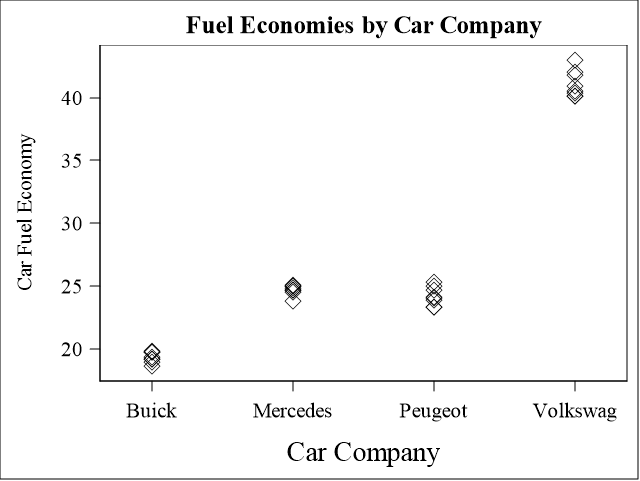
\includegraphics[width = 0.8\textwidth]{dotplot.png}
		\end{center}


		\item Denote the mean fuel economies of cars from Buick $\mu_1$, Mercedes $\mu_2$, Peugeot $\mu_3$ and Volkswagen $\mu_4$.

		$H_0 : \mu_1 = \mu_2 = \mu_3 = \mu_4$

		$H_a :$ at least one $\mu_i$ from $\mu_1, \mu_2, \mu_3, \mu_4$ is different than others.

		Test statistic : $F = 1434.06$

		p-value: $<.0001$

		 we will reject the null hypothesis and conclude there is sufficient evidence that at least one of the mean fuel economies of cars from the four companies is different than the others.

\begin{center}
\begin{tabular}{llllll}
\toprule
Source          & DF & Sum of Squares & Mean Square & F Value & Pr \textgreater F \\
\midrule
Model           & 3  & 2166.460000    & 722.153333  & 1434.06 & \textless.0001    \\
Error           & 28 & 14.100000      & 0.503571    &         &                   \\
Corrected Total & 31 & 2180.560000    &             &         & \\
\bottomrule                  
\end{tabular}
\end{center}



	\item The result of Tukey's HSD method is shown below. From the result we can see that the mean fuel economies of cars from Mercedes and Peugeot, there is no significant difference in the mean fuel economy between these two brands. The mean fuel economy of Volkswagen is significantly different from the others with a higher mean. The mean fuel economy of Buick is also significantly different from the other three with a lower mean.
\begin{center}
	\begin{tabular}{ll}
	\toprule
	Alpha&0.05\\
    Error Degrees of Freedom&28\\
    Error Mean Square&0.503571\\
    Critical Value of Studentized Range&3.86124\\
    Minimum Significant Difference&0.9688\\
    \bottomrule
	\end{tabular}

	\begin{tabular}{llll}
	\toprule
	Tukey Grouping&Mean&N&company\\
	\midrule
A&41.1000&8&Volkswag\\
B&24.7000&8&Mercedes\\
B&24.2000&8&Peugeot\\
C&19.3000&8&Buick\\
\bottomrule
	\end{tabular}
	\end{center}


	\item In the order of $\mu_1,\, \mu_2, \mu_3, \mu_4$, the contrasts should be like this
	\begin{enumerate}
		\item Volkswagen versus the other three companies: $\bm c = (-1/3, -1/3, -1/3, 1)$
		\item Buick versus Mercedes and Peugeot: $\bm c = (1, -1/2, -1/2, 0)$
		\item Mercedes versus Peugeot: $\bm c = (0,1,-1,0)$
	\end{enumerate}

	$(-1/3) \times 1 + (-1/3)\times (-1/2) + (-1/3)\times (-1/2) + 1 \times 0= 0$

	$(-1/3)\times 1 + (-1/3) \times (-1/2) + (-1/3)\times (-1/2) + 1 \times 0= 0$

	$1 \times 0 + (-1/2)\times 1 + (-1/2)\times (-1) + 0 \times 0 = 0$

	Thus these three contracts are orthogonal.


	\item This result means the two contrasts $\mu_4 - (\mu_1 + \mu_2 + \mu_3)/3$ and $\mu_1 - (\mu_2 + \mu_3)/2$ are significantly different from 0, while the contrast $\mu_2 - \mu_3$ is not significantly different from 0. Thus, the mean fuel economy of cars from Volkswagen is significant different from the mean fuel economy of the other three companies; the mean fuel economy of cars from Buick is significantly different than the mean fuel economy of Mercedes and Peugeot; but the mean fuel economy of Mercedes and Peugeot are not significantly different.

\hspace{-5em}
	\begin{tabular}{llllll}
	\toprule
	Contrast & Estimate&Standard Error& Contrast SS	& $F$ Value & Pr $>F$\\
	\midrule
Volkwagen-(Buick + Mercedes + Peugeot)/3&18.3666667&0.28970428&2024.006667&4019.30&$<.0001$\\
Buick-(Mercedes+Peugeot)/2&-5.1500000&0.30727779&141.453333&280.90&$<.0001$\\
Mercedes-Peugeot&0.5000000&0.35481383&1.000000&1.99&0.1698\\
\bottomrule
	\end{tabular}

	
	\item 
	\begin{enumerate}
		\item Independence: the description of the experiment did not indicate how the experiment units are selected. If the cars from the 4 companies are randomly chosen from the population, we can assume they are independent.

		\item Homogeneous variance: The ratio of the largest to smallest company standard deviation is between 2 and 3, and the  Brown and Forsythe's Test fails to reject the null hypothesis of equal variances. So we will conclude the assumption of homogeneous variances is valid.

		\begin{center}
		\begin{tabular}{lllll}
		\toprule
		 & Buick & Mercedes & Peugeot & Volkswagen\\
		 \midrule
		 Std. Dev. & 0.4208834 & 0.4140393 & 0.7425824 & 1.0555973\\
		 \bottomrule
		\end{tabular}

		\begin{tabular}{llllll}
		\toprule
		Source&DF&Sum of Squares&Mean Square&F Value&Pr $> F$\\
		\midrule
        company&3&1.5400&0.5133&2.37&0.0917\\
        Error&28&6.0600&0.2164&&\\
        \bottomrule
		\end{tabular}
		\end{center}

		\item 
		Normal Distribution: The normal quantile plot does not indicate a large amount of deviation from a straight line. So we will conclude the assumption of normality is valid.
		\vspace{\baselineskip}
		\begin{center}
		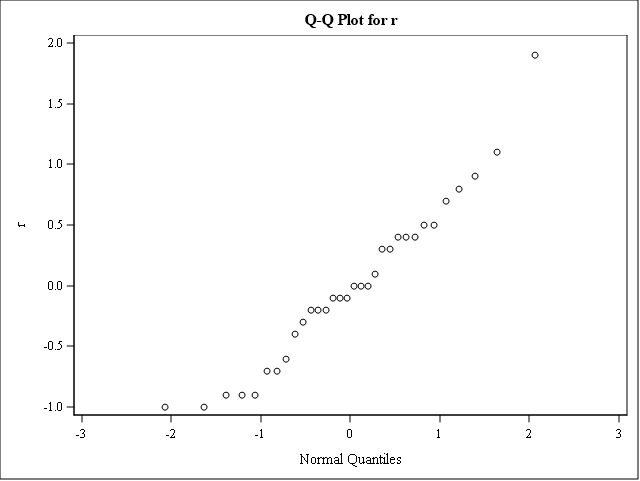
\includegraphics[width = 0.8\textwidth]{qqplot.png}
		\end{center}
	\end{enumerate}
	

		\end{enumerate}
\end{enumerate}
	
	\end{document}